% TODO: \usepackage{graphicx} required
\begin{figure}[h]
	\centering
	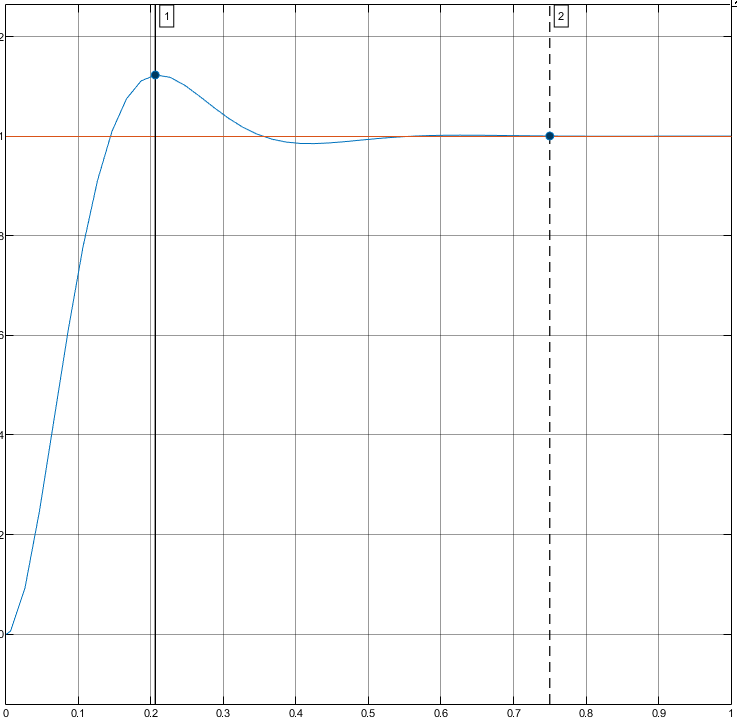
\includegraphics[width=0.4\textwidth]{media/subamortiguado-no-pid}
	\caption{Respuesta del sistema inicial}
	\label{fig:subamortiguado-no-pid}
\end{figure}

% TODO: \usepackage{graphicx} required
\begin{figure}[h]
	\centering
	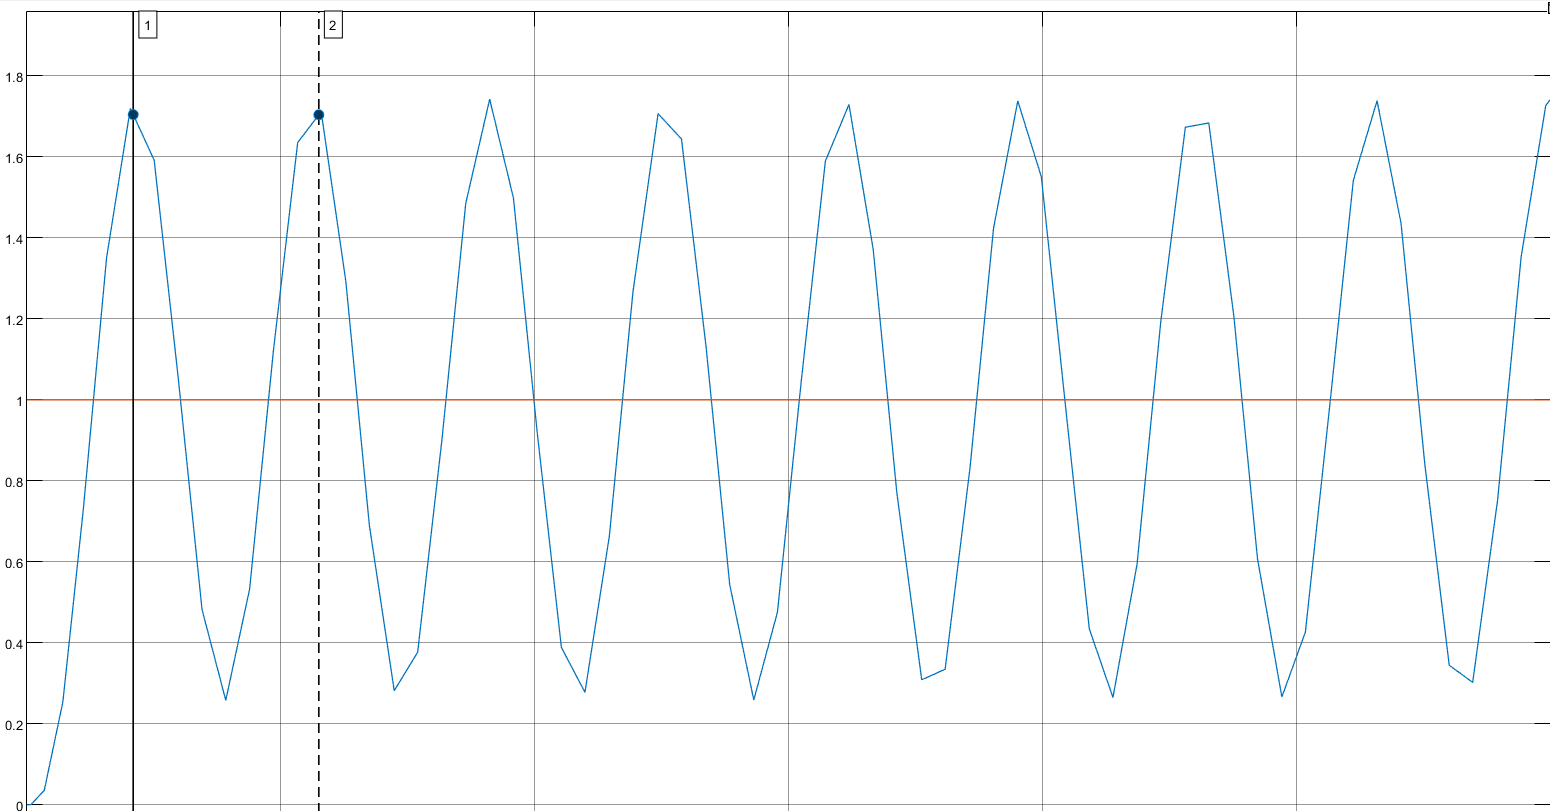
\includegraphics[width=0.4\textwidth]{media/oscilacion_sistema}
	\caption{Oscilación del sistema sub amortiguado}
	\label{fig:oscilacionsistema}
\end{figure}

% TODO: \usepackage{graphicx} required
\begin{figure}[h]
	\centering
	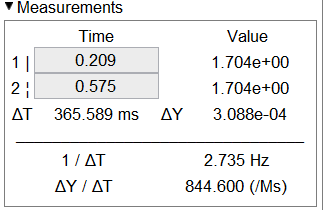
\includegraphics[width=0.4\textwidth]{media/calculo-periodo-oscilacion}
	\caption{Periodo del Oscilación del sistema}
	\label{fig:calculo-periodo-oscilacion}
\end{figure}
